\chapter{Unification of the Fisherian and Neymanian Inferences in Randomized Experiments}\label{chapter::unification-fisher-neyman}
 \chaptermark{Unification of Fisherian and Neymanian Inferences}


Chapters \ref{ch::frt-cre}--\ref{chapter::mpe} cover both the Fisherian and Neymanian inferences for different types of experiments. The Fisherian perspective focuses on the finite-sample exact $p$-values for testing the strong null hypothesis of no causal effects for any units whatsoever, whereas the Neymanian perspective focuses on unbiased estimation with a conservative large-sample confidence interval for the average causal effect. Both of them are justified by the physical randomization which is ensured by the design of the experiments. Because of this, they are both called {\it randomization-based inference} or {\it design-based inference}. Because they concern a finite population of units in the experiments, they are also called {\it finite-population inference}.  They are related but also have distinct features. 

In 1935, Neyman presented his seminal paper on randomization-based inference to the Royal Statistical Society. His paper \citep{neyman1935statistical} was attacked by Fisher in the discussion session. \cite{sabbaghi2014comments} reviewed this famous Neyman--Fisher controversy and presented some new results for this old problem. Instead of going to the philosophical issues, this chapter tries to provide a unified discussion. 



\section{Testing strong and weak null hypotheses in the CRE} 
 \label{sec::strong-weak-cre-frt}
 
 
Let us revisit the treatment-control CRE.  The Fisherian perspective focuses on testing the strong null hypothesis
$$
\HF: Y_i(1) = Y_i(0) \text{ for all units } i=1,\ldots, n.
$$
The FRT delivers a finite-sample exact $p_\frt$ defined in \eqref{eq::exactpvalue}. 
 
 
By duality of the confidence interval and hypothesis testing, the Neymanian perspective gives a test for the  weak null hypothesis
$$
\HN : \tau = 0  \Longleftrightarrow \HN: \bar{Y}(1) = \bar{Y}(0)
$$ 
based on 
$$
t= 
\frac{\hat{\tau} }{  \sqrt{  \hat{V}    } }  .
$$
By the CLT of $\hat\tau$ and the conservativeness of the variance estimator, we have 
$$
t  =   \sqrt{  \frac{ \var(\hat{\tau}) }{ \hat{V} } } \times  \frac{\hat{\tau} }{  \sqrt{  \var(\hat{\tau})   } }    \rightarrow  C \times   \N01 
$$
in distribution, where $C$ is smaller than or equal to $1$ but depends on the unknown potential outcomes. Using $\N01$ quantiles for the studentized statistic $t$, we have a conservative large-sample test for $\HN$. 

Furthermore, \citet{ding2017randomization} show that the FRT with the studentized statistic $t$ has the dual guarantees:
\begin{enumerate}
\item 
 $p_\frt$ is finite-sample exact under $\HF$;
\item
 $p_\frt$ is asymptotically conservative under $\HN$.
\end{enumerate}
Importantly, this is a feature of the studentized statistic $t$. \citet{ding2017randomization} showed that the FRT with other test statistics may not have the dual guarantees. In particular, the FRT with $\hat{\tau}$ may be asymptotically anti-conservative under $\HN$. I give some heuristics below to illustrate the importance of studentization in the FRT. 


Under $\HN$, we have
$$
\hat{\tau} \asim \textsc{N}\left(0,    \frac{S^2(1)}{n_1} + \frac{S^2(0)}{n_0} -  \frac{S^2(\tau)}{n}    \right).
$$
The FRT pretends that the Science Table is $(Y_i, Y_i)_{i=1}^n$ induced by $\HF$, so the randomization distribution of $\hat{\tau} $ is
$$
(\hat{\tau} )^\pi \asim \textsc{N}\left(0,    \frac{s^2}{n_1} + \frac{s^2}{n_0}    \right),
$$
where $(\cdot)^\pi$ denotes the randomization distribution\footnote{$\pi$ is a standard notation for a random permutation.}
 and 
$
s^2 
$
is the sample variance of the observed outcomes. Based on \eqref{eq::frt-algebra-difference-in-means} in Chapter \ref{ch::frt-cre}, we can approximate the asymptotic variance of $(\hat{\tau} )^\pi$ under $\HF$ as
\begin{eqnarray*}
\frac{s^2}{n_1} + \frac{s^2}{n_0} 
& =& \frac{n}{n_1 n_0}  \left\{ 
 \frac{n_1 -1}{ n-1 } \hat S^2(1) + \frac{n_0 - 1}{n-1} \hat S^2(0) + \frac{n_1n_0}{n(n-1)} \hat\tau^2
 \right\} \\
&\approx & \frac{\hat S^2(1) }{n_0} +  \frac{\hat S^2(0) }{n_1} \\ 
&\approx & \frac{  S^2(1) }{n_0} +  \frac{  S^2(0) }{n_1},
\end{eqnarray*}
 which does not match the asymptotic variance of $\hat{\tau} $. Ideally, we should compute the $p$-value under $\HN$ based on the true distribution of $\hat{\tau} $, which, however, depends on the unknown potential outcomes. In contrast, we use the FRT to compute the $p_\frt$ based on the permutation distribution $(\hat{\tau} )^\pi $, which does not match the true distribution of $\hat{\tau} $ under $\HN$ even with large samples. Therefore, the FRT with $\hat\tau$ may not control the type one error rate under $\HN$ even with large samples. 
 
 
Fortunately, the undesired property of the FRT with $\hat\tau$ goes away if we replace the test statistic $\hat{\tau} $ with the studentized version $t$. Under $\HN$, we have
$$
t \asim \textsc{N}(0,  C^2)
$$ 
where $C^2 \leq 1$ with equality holding if $Y_i(1) - Y_i(0) = \tau$ for all units $i=1, \ldots, n$. The FRT pretends that $Y_i(1) = Y_i(0) = Y_i$ for all $i$'s and generates the permutation distribution
$$
t^\pi \asim \textsc{N}(0,  1)
$$
where the variance equals $1$ because the Science Table used by the FRT has zero individual causal effects.  Under $\HN$, because the true distribution of $t$ is more dispersed than the corresponding permutation distribution, the $p_\frt$ based on $t$ is asymptotically conservative. 

%Whether $\HF$ or $\HN$ makes more sense? This is a famous controversy between Neyman and Fisher in a meeting at the Royal Statistical Society, UK \citep{neyman1935statistical, sabbaghi2014comments, Ding:2014}.  
%Recently, \citet{ding2017randomization} advocated using $\hat{\tau} /  \sqrt{  \hat{V}    } $, i.e., the studentized statistic $t$ in Example \ref{eg::studentized-statistic} of Chapter \ref{ch::frt-cre}, in the FRT so that the $p$-value is finite sample exact for $\HF$ and asymptotically valid for $\HN$.  In contrast, using the difference-in-means in the FRT does not have these guarantees. 







 
 
\section{Covariate-adjusted FRTs in the CRE}
 \label{sec::xfrt-cre}
 
Extending the discussion in Section \ref{sec::strong-weak-cre-frt} to the case with covariates, \citet{zhao2020caFRT} recommend using the FRT with the studentized \citet{lin2013}'s estimator:
$$
t_\textsc{L}   =  \frac{  \hat{\tau}_\textsc{L} }{  \sqrt{\hat{V}_\textsc{L}}  },
$$ 
which is the robust $t$-statistic for the coefficient of $Z_i$ in the OLS fit of $Y_i$ on $( 1, Z_i, X_i, Z_i X_i) $. They show that the FRT with $t_\textsc{L} $ has multiple guarantees:
 \begin{enumerate}
\item
 $p_\frt$ is finite-sample exact under $\HF$;
\item
 $p_\frt$ is asymptotically conservative under $\HN$;
\item
 $p_\frt$ is asymptotically more powerful than the FRT with $t$ when $\HN$ does not hold and the covariates are predictive to the outcomes;
\item
the above properties hold even when the linear outcome model is misspecified. 
\end{enumerate}
Similarly, this is a feature of the studentized statistic $t_\textsc{L} $. \citet{zhao2020caFRT} show that other covariate-adjusted FRTs reviewed in Section \ref{sec::covariate-adjusted-frt-intro} may  be either anti-conservative under $\HN$ or less powerful than the FRT with $t_\textsc{L} $ when $\HN$ does not hold.  




\section{A simulation study}
\label{sec::simulation-xfrt-typeoneerror}




Now I use simulation to evaluate the finite-sample properties of the $p_\frt$'s under the weak null hypothesis. I will use the following twelve test statistics.
\begin{enumerate}
\item
The first three test statistics are from the OLS implementation of \citet{Neyman:1923}, including the coefficient of the treatment, the $t$-statistic based on the classic standard error, and the $t$-statistic based on the EHW standard error.

\item
The next three test statistics are based on the pseudo-outcome strategy in Definition \ref{def::pseudo-y-frt}, advocated by \citet{rosenbaum2002covariance}. We first residualize the outcomes by regressing $Y_i$ on $(1,X_i)$, and then obtain the three test statistics similar to the first three.

\item
The next three test statistics are based on the OLS implementation of \citet{fisher1925statistical}, as discussed in Chapter \ref{sec::ancova}.

\item
The final three test statistics are based on the OLS implementation of \citet{lin2013}, as discussed in Chapter \ref{sec::ancova}.
\end{enumerate}

 


Consider a finite population of $n=100$ units subjected to a CRE of size $(n_1, n_0) =(20,80)$.
For each $i  $, we draw a univariate covariate $ X_i $ from Unif$(-1,1)$ and generate potential outcomes as $Y_i(1) \sim \textsc{N}(  X_i ^3 , 1)$ and $Y_i(0) \sim \textsc{N}( - X_i ^3 , 0.5^2)$.
Center the $Y_i(1)$'s and $Y_i(0)$'s  to ensure $\tau= 0$.  
Fix $\{Y_i(1), Y_i(0),  X_i \}_{ i = 1}^{n} $ in simulation. We draw a random permutation of $n_1$ 1's and $n_0$ 0's to obtain the observed outcomes and conduct FRTs. 
The procedure is repeated 500 times, with the $p$-values approximated by 500 independent permutations of the treatment vector in each replication. 



Figure \ref{fig::xfrt-type1error} shows the $p$-values under the weak null hypothesis.
The four robust $t$-statistics, as shown in the last row, are the only ones that preserve the correct type one error rates. 
In fact, they are conservative, which is coherent with the theory. 
All the other eight statistics yield type one error rates greater than the nominal levels and are thus not proper for testing the weak null hypothesis.

 



\begin{sidewaysfigure} 
\centering
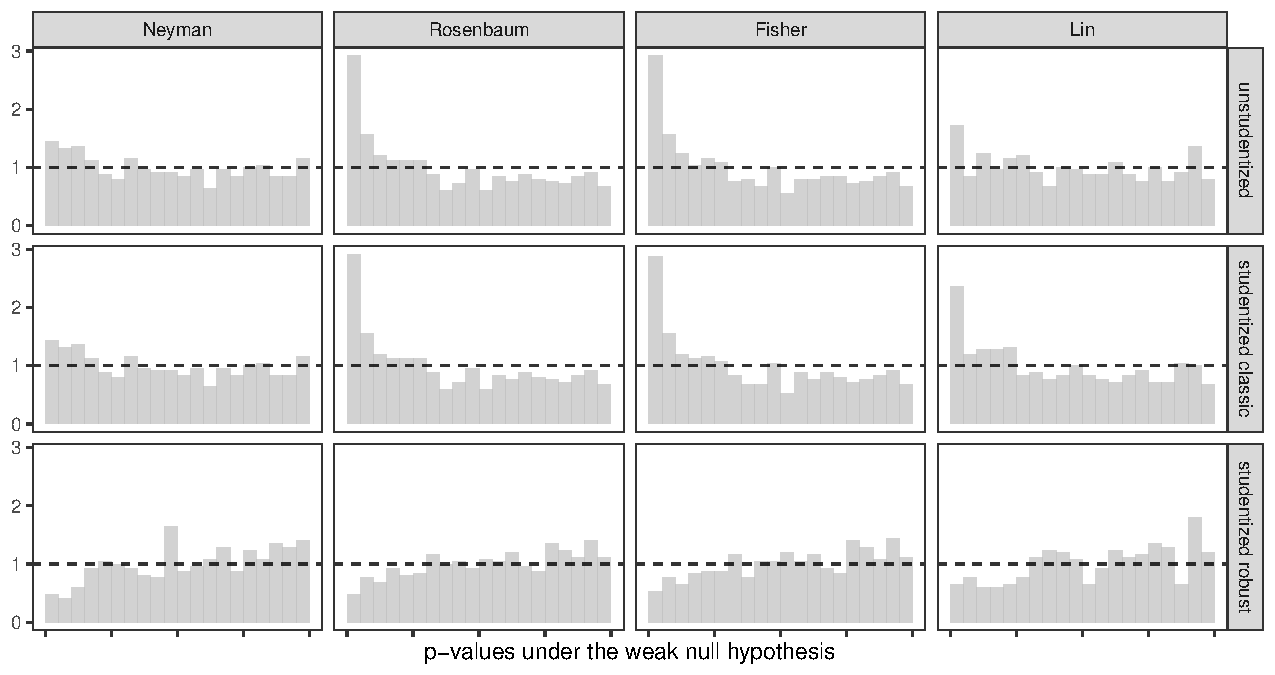
\includegraphics[width = \textwidth]{figures/typeoneerrorXFRT.pdf}
\caption{Histograms of $p_\frt$ under the weak null hypothesis}\label{fig::xfrt-type1error}
\end{sidewaysfigure}










\section{General recommendations}






The recommendations for the SRE parallel those for the CRE if both the strong and weak null hypotheses are of interest. 
Recall the estimators in Chapters \ref{chapter::stratification-poststratification} and \ref{sec::covariate-SRE}. 
Without additional covariates, \citet{zhao2020caFRT} recommend  using the FRT with 
$$
t_\textsc{S} =  \frac{  \hat{\tau}_\textsc{S} }{  \sqrt{\hat{V}_\textsc{S}} } ;
$$ 
with additional  covariates, they recommend using the FRT with 
$$
t_\textsc{L,S} =  \frac{  \hat{\tau}_\textsc{L,S} }{  \sqrt{\hat{V}_\textsc{L,S}} } . 
$$ 


The analysis of ReM is trickier. \citet{zhao2020caFRT} show that the FRT with $t$ does not have the dual guarantees in Section \ref{sec::strong-weak-cre-frt}, but the FRT with $t_\textsc{L}$ still has the guarantees in Section \ref{sec::xfrt-cre}. This highlights the importance of both covariate adjustment and studentization in ReM. 




Similar results hold for the MPE. Without covariates, we recommend using the FRT with the $t$-statistic for the intercept in the OLS fit of $\hat\tau_i$ on $1$; with covariates, we recommend using the FRT with the $t$-statistic for the intercept in the OLS fit of $\hat\tau_i$ on $1$ and $\hat\tau_{X,i}$. Figure \ref{fig::frt-television-mpe} in Chapter \ref{chapter::mpe} are based on these recommended FRTs. 



Overall, the FRTs with studentized statistics are safer choices. When the large-sample Normal approximations to the studentized statistics are accurate, the  $p_\frt$'s are almost identical to the $p$-values based on Normal approximations. When the large-sample approximations are inaccurate, the FRTs at least guarantee valid $p$-values under the strong null hypotheses. This is the recommendation of this book. 



\section{A case study}
\label{sec::case-study-chong}

 

Recall the SRE in \citet{chong2016iron} analyzed in Chapter \ref{sec::ps-chong}. 
I compare the ``soccer'' arm versus the ``control'' arm and the ``physician'' arm versus the ``control'' arm. We also compare the FRTs with and without using the covariate indicating the baseline anemia status. We use their dataset to illustrate the FRTs in the CRE and SRE.  The ten subgroup analyses within the same class levels use the FRTs with $t$ and $t_\textsc{L}$ for the CRE and the two overall analyses averaging over all class levels use the FRTs with $t_\textsc{S}$ and $t_\textsc{L,S}$ for the SRE. 

Table \ref{tb::pv-values-chong} shows the point estimators, standard errors, the $p$-value based on the Normal approximation of the robust $t$-statistics, and the $p$-value based on the FRTs. In most strata, covariate adjustment decreases the standard error since the baseline anemia status is predictive of the outcome. Table \ref{tb::pv-values-chong} also exhibits two exceptions: within class 2, covariate adjustment increases the standard error when comparing ``soccer'' and ``control''; in class 4, covariate adjustment increases the standard error when comparing ``physician'' and ``control''. This is due to the small group sizes within these strata, causing the asymptotic approximation inaccurate. Nevertheless, in these two scenarios, the differences in the standard error are in the third digit.  The $p$-values from the Normal approximation and the FRT are close with the latter being slightly larger in most cases. Based on the theory, the $p$-values based on the FRT should be trusted since it has an additional guarantee of being finite-sample exact under the sharp null hypothesis. This becomes important in this example since the group sizes are quite small within strata. 

\begin{table}
\centering
\caption{Re-analyzing \citet{chong2016iron}'s data. ``\textsc{N}'' corresponds to the unadjusted estimators and tests due to \citet{Neyman:1923}, and ``\textsc{L}'' corresponds to the covariate-adjusted estimators and tests due to \citet{lin2013}.}\label{tb::pv-values-chong}
\begin{subtable}[h]{0.45\textwidth}
\caption{soccer versus control}
    \begin{tabular}{rrrrr}
    \hline 
   &    est & s.e. &$p_\text{Normal}$ & $p_\frt$ \\
       class 1& &&&\\
\textsc{N}  &  0.051 &0.502 &     0.919  & 0.924 \\
\textsc{L}   &    0.050 & 0.489 &     0.919 &  0.929 \\
       class 2& &&&\\
\textsc{N}  &  -0.158 &0.451  &    0.726  & 0.722\\
\textsc{L}   &  -0.176 & 0.452   &   0.698  & 0.700 \\
       class 3& &&&\\
\textsc{N}  &  0.005 &0.403  &    0.990 &  0.989 \\
\textsc{L}   &   -0.096& 0.385 &     0.803&   0.806 \\
       class 4& &&&\\
\textsc{N}  &  -0.492& 0.447  &    0.271 &  0.288 \\
\textsc{L}   &    -0.511& 0.447  &    0.253 &  0.283 \\
       class 5& &&&\\
\textsc{N}  &  0.390& 0.369 &     0.291 &  0.314 \\
\textsc{L}   &   0.443 &0.318  &    0.164  & 0.186 \\
       all& &&&\\
\textsc{N}  &  -0.051 & 0.204  &    0.802 &  0.800 \\
\textsc{L}   &    -0.074& 0.200   &   0.712  & 0.712\\
\hline 
    \end{tabular}
\end{subtable}

\begin{subtable}[h]{0.45\textwidth} 
\caption{physician versus control}
    \begin{tabular}{rrrrr}
    \hline 
   &    est & s.e. &$p_\text{Normal}$ & $p_\frt$ \\
       class 1& &&&\\
\textsc{N}  &  0.567 &0.426  &    0.183 &  0.192 \\
\textsc{L}   &   0.588& 0.418  &   0.160  & 0.174 \\
       class 2& &&&\\
\textsc{N}  &   0.193& 0.438 &     0.659 &  0.666 \\
\textsc{L}   &  0.265& 0.409   &   0.517  & 0.523 \\
       class 3& &&&\\
\textsc{N}  &  1.305& 0.494  &    0.008 &  0.012\\
\textsc{L}   &  1.501& 0.462   &   0.001  & 0.003 \\
       class 4& &&&\\
\textsc{N}  &  -0.273& 0.413  &    0.508 &  0.515 \\
\textsc{L}   &  -0.313& 0.417   &   0.454  & 0.462\\
       class 5& &&&\\
\textsc{N}  & -0.050 &0.379  &    0.895 &  0.912 \\
\textsc{L}   &  -0.067& 0.279  &    0.811 &  0.816 \\
       all& &&&\\
\textsc{N}  &  0.406 & 0.202   &   0.045 &  0.047\\
\textsc{L}   &    0.463 & 0.190   &   0.015  & 0.017 \\
\hline 
    \end{tabular}
\end{subtable}
\end{table}



Figure \ref{fig::randomization-distributions-chong} compares the histograms of the randomization distributions of the robust $t$-statistics with the asymptotic approximations. In the subgroup analysis, we can observe discrepancies between the randomization distributions and $\textsc{N}(0,1)$; averaged over all class levels, the discrepancy becomes unnoticeable. Overall, in this application, the $p$-values based on the Normal approximation do not differ substantially from those based on the FRTs. Two approaches yield coherent conclusions: the video with a physician telling the benefits of iron supplements improved academic performance and the effect was most significant among students in class 3; in contrast, the video with a famous soccer player telling the benefits of the iron supplements did not have any significant effect. 



\begin{sidewaysfigure}
\centering
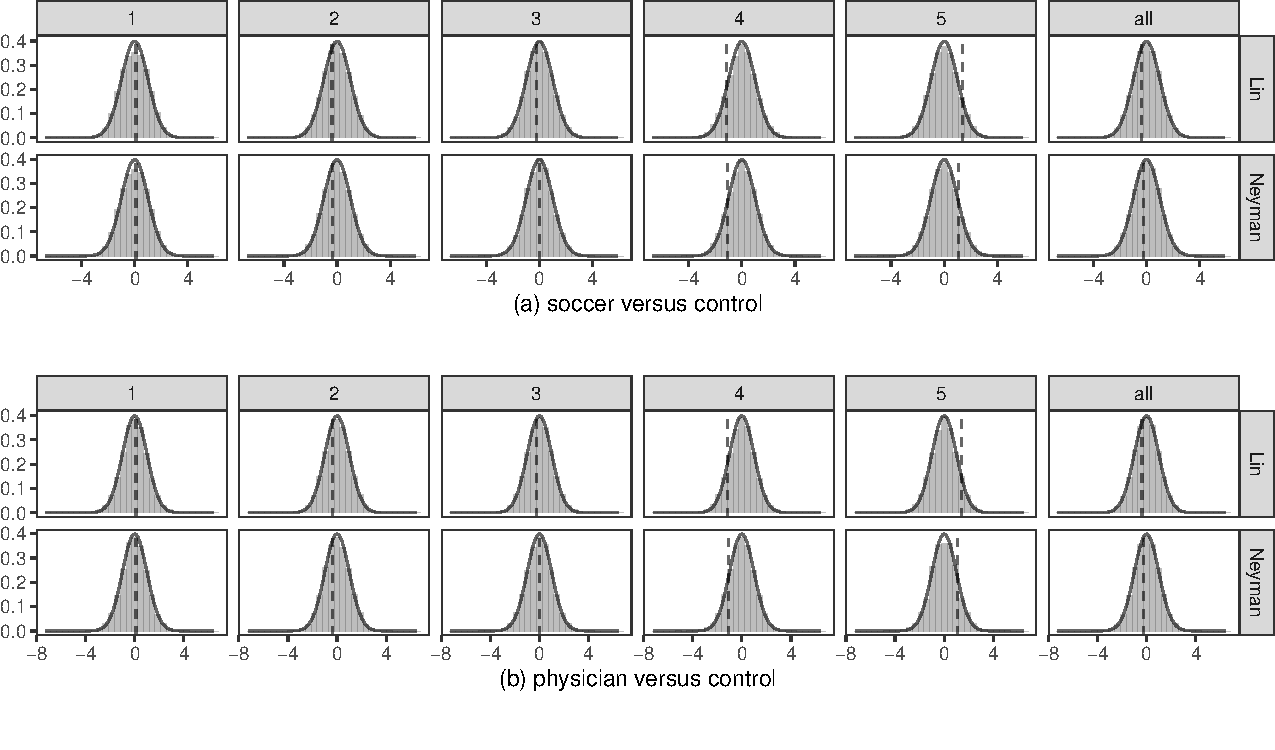
\includegraphics[width = \textwidth]{figures/frt_dist_chong.pdf}
\caption{Re-analyzing \citet{chong2016iron}'s data: randomization distributions with $5\times 10^4$ Monte Carlo draws and the $\N01$ approximations}
\label{fig::randomization-distributions-chong}
\end{sidewaysfigure}


 \section{Homework Problems}


\paragraph{Re-analyzing \citet{angrist2009effects}'s data}\label{para::AL-mpe-fisher}

This is the Fisherian counterpart of Problem \ref{para::AL-mpe-neyman}.
Report the $p_\frt$'s from the FRTs with studentized statistics. 


\paragraph{Replication of \citet{zhao2020caFRT}'s Figure 1}\label{para::zhaoding-xfrt}

\citet{zhao2020caFRT} use simulation to evaluate the finite-sample properties of the $p_\frt$'s from the FRTs with various test statistics. Based on their Figure 1, they recommend using the FRT with $t_\textsc{L,S} $ to analyze the SRE. Replicate their Figure 1. 


\paragraph{Recommended readings}

Using the studentized statistics in permutation tests is not a new idea; see \citet{Janssen97} and \citet{Romano13}. Under the design-based framework, \citet{ding2017randomization} and \citet{wu2018randomization} made the recommendation for multiarmed experiments, and  \citet{zhao2020caFRT} extended the recommendation to covariate adjustment.  

